\documentclass[11pt]{article}
\usepackage{amssymb, amsmath, libertine, hyperref, xcolor, booktabs, enumitem, microtype}
\usepackage[T1]{fontenc}
\usepackage[margin=1in]{geometry}
\usepackage{tikz}
\newcommand{\gridxy}[4]{%
  \foreach \gX in {#1,...,#2} \draw[gray!25] (\gX,#3) -- (\gX,#4);
  \foreach \gY in {#3,...,#4} \draw[gray!25] (#1,\gY) -- (#2,\gY);}
\definecolor{dark-red}{rgb}{0.4,0.15,0.15}
\definecolor{blue-g}{rgb}{0.15,0.28,0.45}
\hypersetup{colorlinks, linkcolor=dark-red, urlcolor=dark-red}
\setlist[enumerate,1]{label=\textbf{(\alph*)}, leftmargin=*, itemsep=7pt, topsep=5pt}
\pagestyle{empty}
\newcommand{\q}[1]{{\color{gray!55!black}\itshape #1}\par\smallskip}
\newenvironment{statement}{\par\color{gray!55!black}}{\par\medskip}
\newcommand{\prob}[1]{\bigskip\noindent\textbf{\large #1}\par\smallskip}

\begin{document}
\begin{center}
{\Large\bfseries Math 111: Calculus \quad Practice Exam 2 --- Solutions}
\end{center}

\medskip
\noindent These are written out in full. On the exam you would not need this much prose ---
but you would need the \emph{reasons}, and every reason here is one that earns marks.

\bigskip\hrule

%%%%%%%%%%%%%%%%%%%%%%%%%%%%%%%%%%%%%%%%%%%%%%%%%%%%%%%%%%%%%%%%%%%%%%%%%%%%%%%%
\prob{1. Structure first}

\begin{statement}
For each function, first say in a few words how it is built (a sum? a product? a quotient? a composition, and of what?), then differentiate it. You need not simplify.
\end{statement}
\begin{enumerate}
\item \q{$f(x) = x^2\cos x$}
$f$ is a \textbf{product} of $x^2$ and $\cos x$. Product rule:
$f'(x) = 2x\cos x - x^2\sin x$.

\item \q{$g(x) = \dfrac{e^x}{x+1}$}
$g$ is a \textbf{quotient}, $e^x$ over $x+1$. Quotient rule:
\[
g'(x) = \frac{e^x(x+1) - e^x\cdot 1}{(x+1)^2} = \frac{x\,e^x}{(x+1)^2}.
\]

\item \q{$h(x) = \sqrt{1+\sin(3x)}$}
$h$ is a \textbf{composition}, twice over: the square root is outside, $1+\sin(3x)$
is inside, and inside \emph{that}, $3x$ sits inside $\sin$. Chain rule, applied from the
outside in:
\[
h'(x) = \frac{1}{2\sqrt{1+\sin(3x)}}\cdot\cos(3x)\cdot 3 = \frac{3\cos(3x)}{2\sqrt{1+\sin(3x)}}.
\]

\item \q{$k(x) = \ln(1+x^2)$}
$k$ is a \textbf{composition}: $\ln$ outside, $1+x^2$ inside. Chain rule:
$k'(x) = \dfrac{1}{1+x^2}\cdot 2x = \dfrac{2x}{1+x^2}$.

\item \q{Find the tangent line to the graph of $f$ at $x=\pi$, and use it to estimate $f(3)$. (You may leave $\pi$ in your answer.)}
$f(\pi) = \pi^2\cos\pi = -\pi^2$ and $f'(\pi) = 2\pi\cos\pi - \pi^2\sin\pi = -2\pi$.
So the tangent line is
\[
L(x) = -\pi^2 - 2\pi\,(x-\pi),
\]
and
\[
f(3)\approx L(3) = -\pi^2 - 2\pi(3-\pi) = \pi^2 - 6\pi \approx -8.98 .
\]
(For comparison, $f(3) = 9\cos 3\approx -8.91$.)
\end{enumerate}

%%%%%%%%%%%%%%%%%%%%%%%%%%%%%%%%%%%%%%%%%%%%%%%%%%%%%%%%%%%%%%%%%%%%%%%%%%%%%%%%
\prob{2. A balloon, a barometer, and two tables}

\begin{statement}
A weather balloon rises. Its altitude $a(t)$, in meters, is recorded every five minutes:
\begin{center}
\begin{tabular}{@{}lrrrrr@{}}
\toprule
$t$ (minutes) & 0 & 5 & 10 & 15 & 20\\
$a(t)$ (m) & 0 & 400 & 750 & 1050 & 1300\\
\bottomrule
\end{tabular}
\end{center}
Air pressure $P(a)$, in kilopascals, depends only on altitude $a$:
\begin{center}
\begin{tabular}{@{}lrrrrr@{}}
\toprule
$a$ (m) & 0 & 500 & 1000 & 1500 & 2000\\
$P(a)$ (kPa) & 101.3 & 95.5 & 90.0 & 84.8 & 79.9\\
\bottomrule
\end{tabular}
\end{center}
The pressure the balloon experiences at time $t$ is $H(t)=P\big(a(t)\big)$. There are no formulas; the tables are all you have.
\end{statement}
It pays to write out the average rates first. For the altitude table, over each
five-minute stretch: $80, 70, 60, 50$ m/min --- the climb is slowing. For the pressure
table, over each 500-m stretch: $-0.0116$, $-0.0110$, $-0.0104$, $-0.0098$ kPa/m --- pressure
falls more slowly the higher you go.

\begin{enumerate}
\item \q{Estimate $a'(10)$, with units. Then give one estimate of $a'(10)$ that is certainly too large and one that is certainly too small, and say what you are assuming about $a'$ in order to be sure.}
Central difference: $a'(10)\approx\dfrac{a(15)-a(5)}{15-5} = \dfrac{1050-400}{10}
= 65$ m/min.

The averages $80,70,60,50$ are decreasing, so $a'$ appears to be decreasing. If it is,
then every instantaneous rate on $[5,10]$ is at least $a'(10)$, so the backward estimate
$\frac{750-400}{5}=70$ m/min is \textbf{too large}; and every rate on $[10,15]$ is at most
$a'(10)$, so the forward estimate $\frac{1050-750}{5}=60$ m/min is \textbf{too small}.
The assumption doing the work is that $a'$ is decreasing throughout $[5,15]$, not just at
the sampled instants.

\item \q{Estimate $P'(750)$, with units. Say in one sentence what the sign of this number means physically.}
$a(10)=750$ lies between the table entries $500$ and $1000$, so the natural estimate
is the secant across them:
\[
P'(750)\approx\frac{P(1000)-P(500)}{1000-500}=\frac{90.0-95.5}{500} = -0.011
\ \text{kPa per meter.}
\]
The sign is negative because pressure \emph{drops} as the balloon rises: each extra meter
of altitude costs about $0.011$ kPa.

\item \q{Estimate $H'(10)$, with units. Explain why the two numbers you combine should be combined the way you combined them --- in terms of what happens to the balloon over the next minute, not by naming a rule.}
$H'(10)\approx P'(750)\cdot a'(10)\approx(-0.011)(65)\approx -0.72$ kPa per minute.

Why multiply: over the next minute the balloon climbs about $65$ meters (that is what
$a'(10)=65$ m/min says). Each of those meters lowers the pressure by about $0.011$ kPa
(that is what $P'(750)$ says). So the pressure the balloon feels drops by about
$65\times0.011\approx0.72$ kPa in that minute. The units agree: (kPa/m)$\times$(m/min)
$=$ kPa/min, and the meters cancel exactly because the first rate is \emph{per meter of
altitude} and the second \emph{produces} meters of altitude.

\item \q{A classmate computes $H'(10)$ as $P'(10)\cdot a'(10)$. Say precisely what is wrong, and why the number $P'(10)$ is not even the kind of quantity that belongs here.}
$P'(10)$ is the rate of change of pressure at an \emph{altitude} of $10$ meters,
because $P$ is a function of altitude, not time. The balloon is not at $10$ m at time $10$;
it is at $750$ m. The derivative of the outside function has to be evaluated at the inside
function's value, $a(10)=750$, not at the time $10$. Beyond the wrong number, $P'(10)$
answers a question nobody asked --- what happens to pressure near the ground --- and so
cannot be the right factor regardless of its value.
\end{enumerate}

%%%%%%%%%%%%%%%%%%%%%%%%%%%%%%%%%%%%%%%%%%%%%%%%%%%%%%%%%%%%%%%%%%%%%%%%%%%%%%%%
\newpage
\prob{3. A melting snowball}

\begin{statement}
A snowball is melting. Assume it stays a perfect sphere, and that its volume is decreasing at a steady $2$ cubic centimeters per minute. Recall $V=\frac43\pi r^3$ and surface area $S=4\pi r^2$.
\end{statement}
\begin{enumerate}
\item \q{Draw and label a picture, and write down, with units, every rate you know and the rate you want.}
A sphere of radius $r$ (cm), with $r$ changing in time. Known: $\dfrac{dV}{dt}=-2$
cm$^3$/min (negative because the volume is decreasing). Wanted: $\dfrac{dr}{dt}$ when
$r=3$ cm, and then $\dfrac{dS}{dt}$ at the same moment.

\item \q{How fast is the radius shrinking at the moment the radius is $3$ cm?}
From $V=\frac43\pi r^3$, differentiating with respect to time (chain rule, since
$r$ depends on $t$):
\[
\frac{dV}{dt} = 4\pi r^2\,\frac{dr}{dt}
\qquad\Longrightarrow\qquad
\frac{dr}{dt} = \frac{1}{4\pi r^2}\,\frac{dV}{dt} = \frac{-2}{4\pi r^2}.
\]
At $r=3$: $\dfrac{dr}{dt} = \dfrac{-2}{36\pi} = -\dfrac{1}{18\pi}\approx -0.018$ cm/min.
The radius is shrinking by about two hundredths of a centimeter each minute.

\item \q{How fast is the surface area shrinking at that moment?}
From $S=4\pi r^2$: $\dfrac{dS}{dt} = 8\pi r\,\dfrac{dr}{dt}$. At $r=3$, using (b):
\[
\frac{dS}{dt} = 8\pi\cdot3\cdot\Big(-\frac{1}{18\pi}\Big) = -\frac{24}{18} = -\frac43
\ \text{cm}^2\text{/min.}
\]
(Equivalently, $\frac{dS}{dt} = \frac{2}{r}\frac{dV}{dt}$, which is a tidy general fact.)

\item \q{Is the radius shrinking faster or slower when the snowball is smaller? Answer from your formula in (b), then say in a sentence why that makes physical sense.}
From (b), $\dfrac{dr}{dt} = -\dfrac{2}{4\pi r^2}$: the magnitude grows as $r$
shrinks. So the radius shrinks \textbf{faster} when the snowball is smaller. Physically,
the same $2$ cm$^3$ of ice is lost each minute, and on a small sphere that volume is a
thicker shell than on a big one --- the surface area $4\pi r^2$ over which the loss is
spread is smaller, so each minute's loss bites deeper into the radius.
\end{enumerate}

%%%%%%%%%%%%%%%%%%%%%%%%%%%%%%%%%%%%%%%%%%%%%%%%%%%%%%%%%%%%%%%%%%%%%%%%%%%%%%%%
\prob{4. All about $f'$}

\begin{statement}
A function $f$ is differentiable everywhere, and its derivative is $f'(x) = (x-2)(x+1)^2$. You are not told $f$ itself.
\end{statement}
\begin{enumerate}
\item \q{Find all critical numbers of $f$.}
$f'$ is a polynomial, so it is defined everywhere; the critical numbers are where
$f'(x)=0$: $\boxed{x=-1}$ and $\boxed{x=2}$.

\item \q{Make a sign chart for $f'$, and use the first derivative test to classify each critical number as a local maximum, a local minimum, or neither. Justify each from the chart.}
The factor $(x+1)^2$ is never negative, so the sign of $f'$ is the sign of $x-2$:

\smallskip
\begin{center}
\begin{tabular}{@{}lcccc@{}}
\toprule
 & $x<-1$ & $-1<x<2$ & $x>2$ \\
\midrule
$x-2$ & $-$ & $-$ & $+$ \\
$(x+1)^2$ & $+$ & $+$ & $+$ \\
$f'$ & $-$ & $-$ & $+$ \\
\bottomrule
\end{tabular}
\end{center}
\smallskip

At $x=2$, $f'$ changes from negative to positive: $f$ falls, then rises, so $f$ has a
\textbf{local minimum} at $2$. At $x=-1$, $f'$ is negative on both sides: no sign change,
so \textbf{neither} --- $f$ is decreasing through $x=-1$.

\item \q{Compute $f''$ and apply the second derivative test at each critical number. Where the test is silent, say so, and say which test settles the matter.}
Product rule: $f''(x) = (x+1)^2 + (x-2)\cdot2(x+1) = (x+1)\big[(x+1)+2(x-2)\big]
= (x+1)(3x-3) = 3(x+1)(x-1)$.

At $x=2$: $f''(2) = 3\cdot3\cdot1 = 9>0$, so $f$ is concave up there and the second
derivative test confirms the \textbf{local minimum}. At $x=-1$: $f''(-1)=0$, so the test
is \textbf{silent} --- it gives no information either way. The first derivative test in
(b) settles it: no extremum.

\item \q{A classmate writes: ``$f'(-1)=0$, and $f'$ is negative on both sides of $-1$, so the graph of $f$ turns around at $x=-1$ and $f$ has a local maximum there.'' Find the first wrong step, say why it is wrong, and describe what the graph of $f$ actually does near $x=-1$.}
The first wrong step is ``\textbf{so the graph of $f$ turns around at $x=-1$}.''
A function turns around where its derivative \emph{changes sign}; a derivative that is
negative on both sides of a point describes a function that is falling on both sides, which
is the opposite of turning around. What actually happens: $f$ decreases as it approaches
$x=-1$, flattens out for an instant (slope exactly $0$), and keeps decreasing. Think of
$-(x+1)^3$ near $-1$. There is no local maximum, and no local minimum either.

\item \q{On axes of your own, sketch a possible graph of $f$ on $[-3,4]$, consistent with everything above. Mark the critical points.}
A sketch consistent with all of the above: decreasing on $(-\infty,2)$ with a flat
step at $x=-1$ (concave down to the left of $-1$ and concave up between $-1$ and $1$,
since $f''$ changes sign at $\pm1$), a minimum at $x=2$, increasing after. The vertical
position is free, since $f$ is only known up to a constant.

\smallskip
\begin{center}
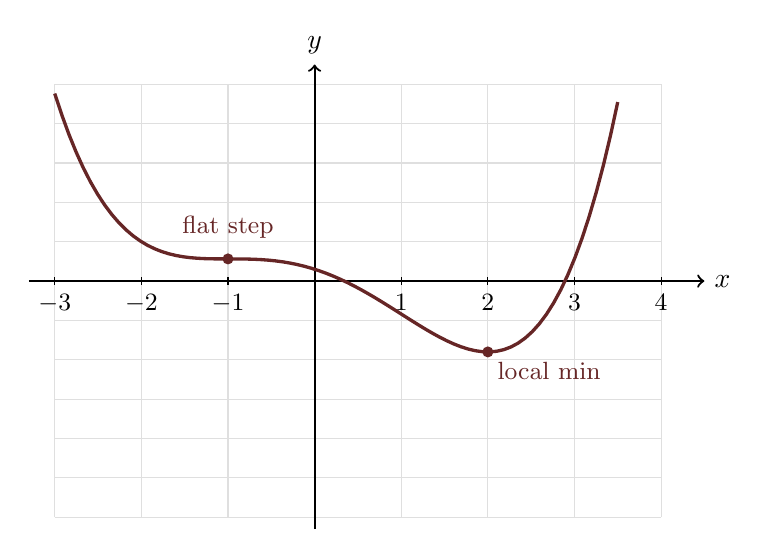
\begin{tikzpicture}[x=1.1cm,y=0.5cm]
  \gridxy{-3}{4}{-6}{5}
  \draw[->,thick] (-3.3,0) -- (4.5,0) node[right] {$x$};
  \draw[->,thick] (0,-6.3) -- (0,5.5) node[above] {$y$};
  \foreach \x in {-3,-2,-1,1,2,3,4} \draw (\x,0.1) -- (\x,-0.1) node[below,font=\small] {$\x$};
  % f = x^4/4 - 2x^3/3 ... antiderivative of (x-2)(x+1)^2 = x^3 - 3x - 2: F = x^4/4 - 3x^2/2 - 2x, scaled
  \draw[very thick, dark-red, domain=-3:3.5, samples=80] plot (\x,{0.35*((\x)^4/4 - 1.5*(\x)^2 - 2*\x) + 0.3});
  \fill[dark-red] (-1,{0.35*(0.25-1.5+2)+0.3}) circle (2pt) node[above=4pt,font=\small] {flat step};
  \fill[dark-red] (2,{0.35*(4-6-4)+0.3}) circle (2pt) node[below right,font=\small] {local min};
\end{tikzpicture}
\end{center}
\end{enumerate}

\end{document}
